\chapter{Validation}
\label{ch:validation}
Nous désirons mesurer deux aspects de notre programme : la qualité des stratégies décrites dans le sujet de \ac{TP} et la complexité de chaque algorithme. Pour cela, nous avons mis en place un championnat qui oppose différentes configurations, ainsi que des mesures de complexité pour chaque algorithme. 


\section{Mesure de complexité : Exploration de l'arbre de jeu}
\label{sec:game_tree_exploration}
Nous comparons ici la complexité en temps et en nombre de nœuds explorés. Nous avons mesuré ces deux aspects sur 24 configurations. Elles correspondent à un affrontement entre soit Minimax, soit Alpha-Beta contre un joueur aléatoire avec une profondeur de recherche de 2, 4 et 6, sur différentes stratégies.


\begin{table}[H]
    \centering
    \caption{NegamaxAlphaBeta/Negamax Analyse comparative à travers les profondeurs et les stratégies en temps de calcul}
    \resizebox{0.9\textwidth}{!}{% Resize table to fit within the text width, keeping aspect ratio
        \begin{tabular}{
            @{}
            >{\raggedright\arraybackslash}p{1cm}
            >{\raggedright\arraybackslash}p{4cm}
            S
            S
            S
            @{}
            }
            \toprule
            \textbf{Depth} & \textbf{Strategy} & {\textbf{Mean}} & {\textbf{Std}} \\
            \midrule
            \multicolumn{4}{c}{\textbf{Depth 2}} \\
            \midrule
                           & Positional                  & {74.10\% (0.03 vs 0.04)}    & {198.71\% (0.02 vs 0.01)}  \\
                           & Absolute                    & {86.94\% (0.01 vs 0.02)}    & {208.26\% (0.02 vs 0.01)}  \\
                           & Mobility                    & {54.55\% (0.06 vs 0.12)}    & {83.37\% (0.02 vs 0.03)}   \\
                           & Mixed (thresholds=[30, 55]) & {67.22\% (0.06 vs 0.08)}    & {140.54\% (0.04 vs 0.03)}  \\
            \midrule
            \multicolumn{4}{c}{\textbf{Depth 4}} \\
            \midrule
                           & Positional                  & {14.56\% (0.90 vs 6.21)}    & {14.38\% (0.30 vs 2.06)}   \\
                           & Absolute                    & {24.09\% (0.51 vs 2.10)}    & {16.92\% (0.19 vs 1.15)}   \\
                           & Mobility                    & {13.04\% (1.50 vs 11.52)}   & {11.27\% (0.49 vs 4.38)}   \\
                           & Mixed (thresholds=[30, 55]) & {15.93\% (1.17 vs 7.34)}    & {12.67\% (0.40 vs 3.18)}   \\
            \midrule
            \multicolumn{4}{c}{\textbf{Depth 6}} \\
            \midrule
                           & Positional                  & {8.45\% (35.20 vs 416.65)}  & {2.60\% (2.82 vs 108.49)}  \\
                           & Absolute                    & {12.23\% (20.14 vs 164.64)} & {18.39\% (13.95 vs 75.87)} \\
                           & Mobility                    & {2.83\% (39.32 vs 1390.49)} & {1.03\% (7.65 vs 745.69)}  \\
                           & Mixed (thresholds=[30, 55]) & {3.17\% (17.34 vs 546.98)}  & {4.36\% (5.04 vs 115.61)}  \\
            \bottomrule
        \end{tabular}
    }
\end{table}

L'unité est la seconde. Nous avons mesuré le temps de calcul pour chaque partie jouée.


\subsection{Nombre de nœuds explorés}
\label{subsec:node_explored}
Nous avons mesuré à chaque coup des joeurs, le nombre de nœuds explorés. Nous pouvons donc comparer chaque algorithme sur un graphe pour chaque profondeur donnée\footnote{Chaque figure est disponible séparément dans les appendices.}.

\begin{figure}[H]
    \centering
    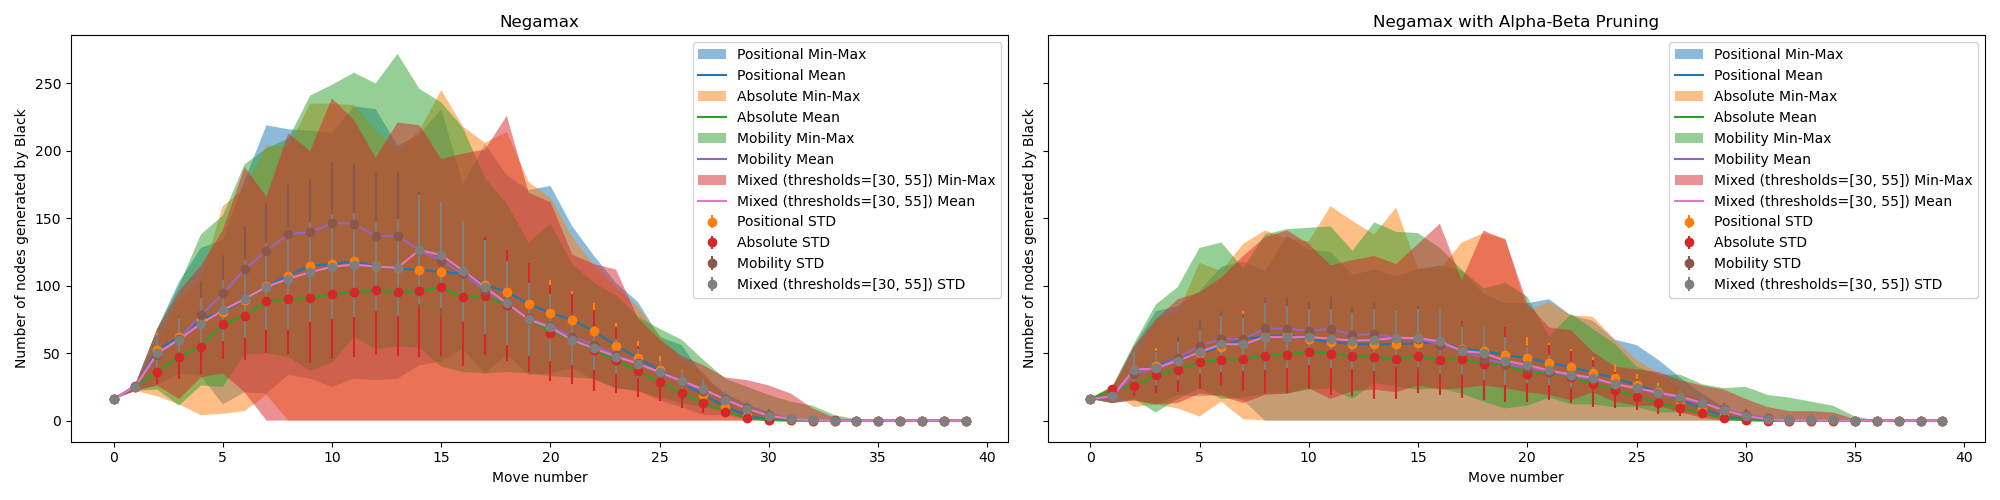
\includegraphics[width=\textwidth]{ressources/Number of nodes generated by Black_depth_2_combined.png}
    \caption{Nombre de nœuds explorés par Minimax et Alpha-Beta en profondeur 2.}
    \label{fig:complexity_node_explored-2}
\end{figure}

\begin{figure}[H]
    \centering
    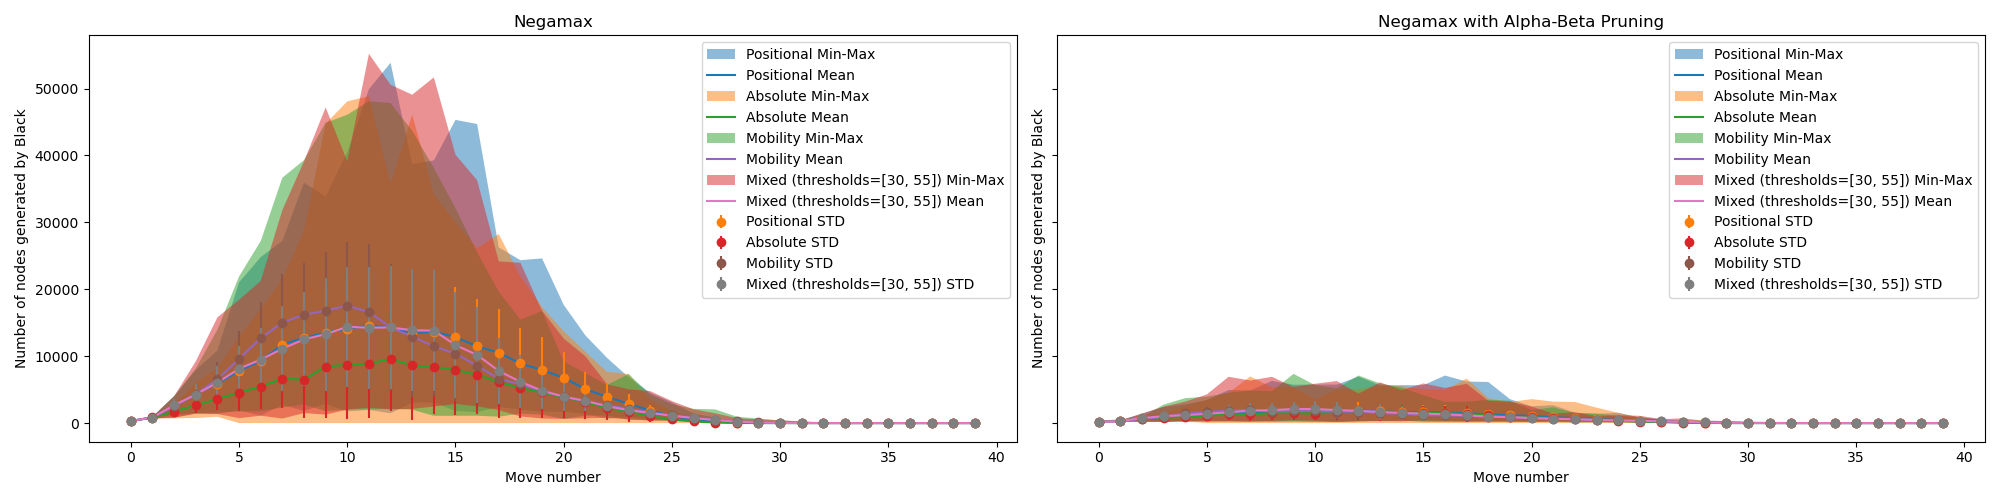
\includegraphics[width=\textwidth]{ressources/Number of nodes generated by Black_depth_4_combined.png}
    \caption{Nombre de nœuds explorés par Minimax et Alpha-Beta en profondeur 4.}
    \label{fig:complexity_node_explored-4}
\end{figure}

\begin{figure}[H]
    \centering
    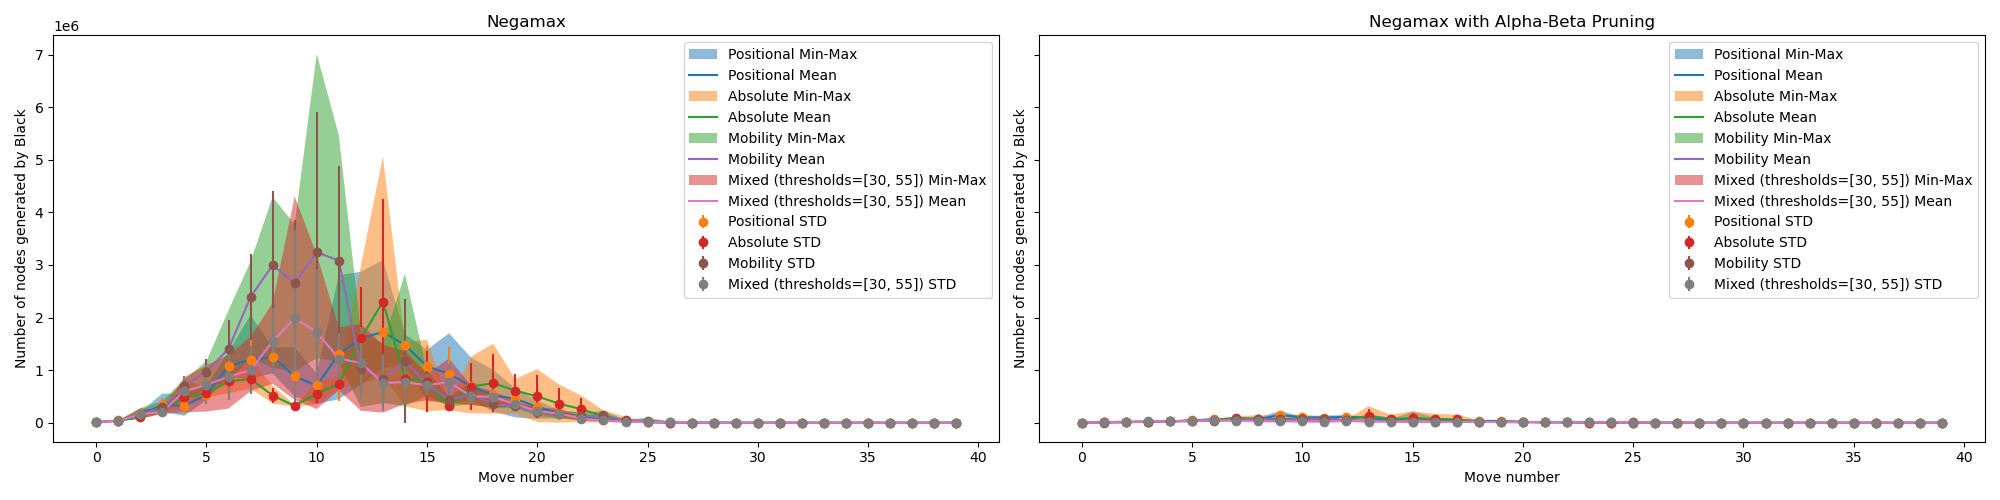
\includegraphics[width=\textwidth]{ressources/Number of nodes generated by Black_depth_6_combined.png}
    \caption{Nombre de nœuds explorés par Minimax et Alpha-Beta en profondeur 6.}
    \label{fig:complexity_node_explored-6}
\end{figure}

Dans un tableau récapitulatif, nous pouvons observer le nombre moyen de nœuds explorés par Minimax et Alpha-Beta pour chaque profondeur. Les résultats sont présentés dans le tableau \ref{tab:node_explored_summary}.

\begin{table}[H]
    \centering
    \caption{NegamaxAlphaBeta/Negamax Analyse comparative à travers les profondeurs et les stratégies}
    \resizebox{\textwidth}{!}{% Resize table to fit within the text width, keeping aspect ratio
        \begin{tabular}{
            @{}
            >{\raggedright\arraybackslash}p{1cm}
            >{\raggedright\arraybackslash}p{4cm}
            S
            S
            S
            @{}
            }
            \toprule
            \textbf{Depth} & \textbf{Strategy}           & {\textbf{Max of Maxs}} & {\textbf{Mean of Means}} & {\textbf{Mean of Stds}} \\
            \midrule
            \multicolumn{5}{c}{\textbf{Depth 2}}                                                                                       \\
            \cmidrule(lr){1-5}
                           & Positional                  & 58.80\%                & 57.52\%                  & 65.20\%                 \\
                           & Absolute                    & 64.90\%                & 55.79\%                  & 63.92\%                 \\
                           & Mobility                    & 54.04\%                & 53.95\%                  & 60.26\%                 \\
                           & Mixed (thresholds=[30, 55]) & 61.09\%                & 58.35\%                  & 62.72\%                 \\
            \midrule
            \multicolumn{5}{c}{\textbf{Depth 4}}                                                                                       \\
            \cmidrule(lr){1-5}
                           & Positional                  & 13.19\%                & 14.77\%                  & 16.35\%                 \\
                           & Absolute                    & 14.27\%                & 21.19\%                  & 17.92\%                 \\
                           & Mobility                    & 15.29\%                & 14.06\%                  & 14.30\%                 \\
                           & Mixed (thresholds=[30, 55]) & 12.54\%                & 15.76\%                  & 15.56\%                 \\
            \midrule
            \multicolumn{5}{c}{\textbf{Depth 6}}                                                                                       \\
            \cmidrule(lr){1-5}
                           & Positional                  & 7.15\%                 & 6.96\%                   & 6.66\%                  \\
                           & Absolute                    & 6.26\%                 & 7.67\%                   & 10.21\%                 \\
                           & Mobility                    & 1.93\%                 & 2.98\%                   & 2.56\%                  \\
                           & Mixed (thresholds=[30, 55]) & 1.84\%                 & 3.07\%                   & 2.77\%                  \\
            \bottomrule
        \end{tabular}
    }
    \label{tab:node_explored_summary}
\end{table}

\section{Championnat : Comparaison des algorithmes}
\label{sec:championship}

